\documentclass[a4paper,10pt, 5p]{elsarticle}
\usepackage[utf8]{inputenc}
\usepackage{amsmath}
\usepackage{amssymb}{}
\usepackage{amsthm}
\usepackage{enumerate}
\usepackage{hyperref}
\usepackage{listings}
\usepackage{booktabs}
\usepackage{siunitx}
\usepackage{graphicx}
\usepackage{cleveref}
\usepackage{changes}
\definechangesauthor[color=orange]{SDIV}
\begin{document}
    \author{SDIV, FPA, DGS, GASV}
    \title{Optimal constant picewise vaccination policies for COVID-19}
    \begin{abstract}
      
      BACKGROUND.

      FINDINGS.
      
      IMPLICATIONS.
    \end{abstract}
    \maketitle
    \section{Introduction}
      In late December 2019, a new virus's appearance is reported in Wuhan City,
Hubei Province, China. Called SARS-CoV2, it is the virus that causes the 2019
corona virus disease (COVID-19) and that, very quickly since its appearance,
has spread throughout much of the world, causing severe problems to health
systems of all the countries in which it is present \cite{Who12020}. On March
11, 2020, the World Health Organization declared the epidemic by COVID-19 as a
pandemic when there were around 118,000 cases distributed in 114 countries, and
approximately 4,291 deaths \cite{Who512020}. In Latin America, the first
detected case of COVID-19 occurred in Brazil on February 26, and in Mexico, the
first case was reported on February 27, quickly spreading throughout the
country \cite{Ajrm2020,Acuna2020}.

Due to the absence of successful treatment and vaccines,
several non-pharmaceutical interventions (NPIs) have been implemented in all the
countries where the disease is present, with quarantine, isolation, and social
distancing being the main ones \cite{Wilder2020,Guner2020,Liu2020_2}. Despite
the measures that different governments have taken to mitigate the epidemic, it
has not been controlled in most places, which may be due to the relaxation of
mitigation measures. At the date of writing this work, the upturn or regrowth
in the number of cases in some countries around the world has been observed. In
some places, this behavior is referred to as "second wave". On the other hand,
since the new coronavirus appearance, the international scientific community
has been working to understand the virus nature. They mainly focus on the
spreading mechanisms between individuals, and developing vaccines and
treatments to reduce the number of infections and fatality cases. To get a
clearer understanding of different vaccination strategies and their
consequences on the number of infected individuals, mathematical models have
taken a leading role.

    The use of various mathematical tools such as SIR and SEIR models has
helped to  describe epidemics properties around the globe. These models have
been used to estimate the basic reproductive number associated with the disease
and also different parameters involved in its spread
\cite{Wang2020,Liu2020,Sarkar2020,Hong2020}. Another use of this kind of model
has been addressed to propose and evaluate the effect of various control
measures classified as NPIs
\cite{Acuna2020,Marimuthu2020,Liu2020,Shaikh2020,DeVisscher2020}.

    Currently, vaccine development for COVID-19 is at an advanced stage. It is
believed that their distribution will begin in early 2021. However, we
consider that, in addition to the vaccine's existence, it is necessary to
have a good vaccination strategy. A widely used tool to address this
question is the optimal control theory. This mathematical tool is useful to
propose scenarios in which the vaccine's application minimizes the damage
caused by the disease and its application cost. Some results about it have
been applied to control other diseases for humans and animals
\cite{Asano2008,Rodrigues2014,Tchuenche2011,Malik2016,Jaberi2014}. Optimal
control theory has also been used in COVID-19 studies. Most efforts have
been invested in finding optimal strategies to evaluate the impact of
non-pharmaceutical interventions
\cite{Madubueze2020,Perkins2020,Ullah2020}. Optimal control strategies have
also being considered in vaccination \cite{Barbosa2020}. In this work, the
authors took their optimization based on a basic compartmental model for
COVID-19. In their model, deaths due to disease are not considered and
vaccination is applied only to susceptible individuals.  \unsure{NO SE VE
    LA DIFERENCIA RESPECTO A NUESTRO TRABAJO, EL QUE NO CONSIDEREN MUERTE NO LO
    HACE TAN DIFERENTE. RECUERDO QUE SAÚL MENCIONÓ ALGO SOBRE QUE LA FORMA DE
    HACER CONTROL ES DISTINTA. O DE PLANO NO HAY? JAJA....Ohh pues...dejame
    ser! estoy en eso!}

In this work, we present a mathematical model to describe the transmission and some vaccination dynamics of COVID-19. Mainly, we focus on using optimal control theory to obtain vaccination strategies in a homogeneous population. Our main objective is to minimize the disability-adjusted life year (DALY) \cite{WhoDALY}. This quantity is used by the World Health Organization (WHO) to quantify the burden of disease from mortality and morbidity, which is given by the sum of the years of life lost (YLL) and years lost due to disability (YLD). This work's objective is framed within the context of the WHO strategic advisory group of experts (SAGE) on immunization working group on COVID-19 vaccines \cite{sage2020}.

Development of COVID-19 vaccines is a major challenge these days. Some research efforts in this direction can be found in \cite{Belete2020,Kaur2020}. In Mexico, some of the considered vaccines to be applied to the population are Adenovirus Type 5 Vector (Ad5-nCoV) by Cansino Biologics, AZD1222 by AstraZeneca and BNT162b2 by Pfizer and BioNTech. At the current date, these and other vaccines are on the testing phase (phase 3) and there are still some questions about the efficacy of the vaccines. In the United States, an appropriate vaccine to be applied needs to show firm evidence that it protects at least half of those inoculated \cite{Shah2020}. At this stage, there are no conclusive results about the efficacy of the vaccines. Also, current work is the immunity time the vaccines will provide to people.

Our work is divided into the following sections. In Section 2, we present our mathematical model, which includes preventive vaccine dynamics. Section 3 includes an analysis of the vaccination reproductive number. Section 4 presents our numerical results regarding optimal vaccination policies. It is important to stress that, with the objective of study COVID-19 dynamics in a specific city and have a set of baseline parameters values, we used the Mexico City plus Mexico state COVID-19 data to estimate some proposed model parameters. We end this work with a conclusions and discussions section.
    \section{Covid-19 spread dynamics}
      
In this section, we formulate our baseline mathematical model,
which additionally to the transmission dynamics, includes vaccination.
In order to build our  model, we follow the classical Kermack-McKendrick
approach. \Cref{Fig:SchemeModel} shows the compartmental diagram of
our mathematical model.
\begin{figure*}[tbh]
    \centering
    \includegraphics[scale = 1]{SchemeModel_0211_v3.pdf}
    \caption{%
        Compartmental diagram of COVID-19 transmission dynamics which
        including vaccination dynamics. Here, there are seven different classes:
        Susceptible $(S)$, exposed $(E)$, symptomatic infected $(I_S)$, asymptomatic
        infected $(I_A)$, recovered $(R)$, death $(D)$ and vaccinated $(V)$
        individuals. It is important to mention that $I_{S}$ represents the
        proportion of symptomatic individuals who will later report
        to some health medical center.}
    \label{Fig:SchemeModel}
\end{figure*}

Information about reinfection dynamics on COVID-19
disease is unclear to date. However, to explore some scenarios related
to this dynamic, we assume that reinfection is possible after a period
of time. On the other hand, we model the vaccination process considering
some assumptions: i) Vaccination is applied to all the alive individuals
except those in the symptomatic class. In this situation, vaccines are
applied indiscriminately over individuals on the $S$, $E$, $I_A$, and
$R$ classes; ii) the vaccine has preventive nature, that is, only
reflected in the susceptible individuals $(S)$; iii) people will only get
one vaccine during the campaign, and iv) vaccines do not necessarily have
a hundred percent of effectivity, which implies that some vaccinated people
can get the disease. We denote the effectivity rate by $\epsilon$.
Based on these assumptions our model becomes
\begin{equation}\label{model1}
    \begin{aligned}
        S'(t) &= \mu \bar{N}-\frac{\beta_S I_S +
            \beta_AI_A}{\bar{N}}S - (\mu+\lambda_V)S +
        \delta_V V+ \delta_R R
        \\
        E'(t) &= \frac{\beta_S I_S + \beta_AI_A}{\bar{N}}S+
        (1-\epsilon) \frac{\beta_S I_S+\beta_AI_A}{\bar{N}}V-(\mu+\delta_E) E
        \\
        I'_S(t) &=
        p \delta_E E-(\mu+\alpha_S) I_S
        \\
        I'_A(t) &= (1-p) \delta_E E-(\mu+\alpha_A) I_A
        \\
        R'(t)&= (1-\theta) \alpha_S I_S +
        \alpha_A I_A-(\mu+\delta_R) R
        \\
        D'(t) &= \theta \alpha_S I_S
        \\
        V'(t) &= \lambda_V S-(1-\epsilon)
        \frac{\beta_S I_S + \beta_AI_A}{\bar{N}}V - (\mu+\delta_V) V
        \\
    \end{aligned}
\end{equation}
%
where $\bar{N}(t)=S(t)+E(t)+I_S(t)+I_A(t)+R(t)+V(t)$ and
$N=\bar{N}+D$. Additionally, we include the equations
\begin{equation}
    \label{eqn:model1_counters}
    \begin{aligned}
        X'(t) &=
        \lambda_V(S + E + I_A + R)
        \\
        Y'_{I_S}(t) &=p
        \delta_E E,
    \end{aligned}
\end{equation}
where $X(t)$ and $Y_{I_S}(t)$ represent the cumulative doses at time $t$,
and the cumulative incidence at time $t$, respectively.
Parameters description of system in \Cref{model1} is provided
in \Cref{table:parametermodel}.

\begin{table*}[tbh]
    \centering
    \begin{tabular}{cl}
        \toprule
        Parameter & Description
        \\
        \midrule
        $\mu$ &  Natural death rate
        \\
        $\beta_S$ & Infection rate between susceptible and symptomatic infected
        \\
        $\beta_A$ & Infection rate between susceptible and asymptomatic infected
        \\
        $\lambda_V$ & Vaccination rate
        \\
        $\delta_{V}^{-1}$ & Immunity average time by vaccination
        \\
        $\epsilon$ &  Vaccine efficacy
        \\
        $\delta_{E}^{-1}$ & Average time of the incubation period \\
        $p$ & Proportion of symptomatic individuals  \\
        $\alpha_{S}^{-1}$ &  Average output time of symptomatic
        individuals due to death or recovery  \\
        $\theta$ & Proportion of symptomatic individuals who die due to
        the disease \\
        $\alpha_{A}^{-1}$
        & Recovery average time of asymptomatic individuals
        \\
        $\delta_{R}^{-1}$
        &  Immunity average time by disease
        \\
        \bottomrule
    \end{tabular}
    \caption{Parameters definition of system in \Cref{model1}.}
    \label{table:parametermodel}
\end{table*}

\subsection{Baseline parameters value and initial conditions}
It is now necessary to define a set of baseline parameter
values to explore some scenarios of interest. In the present work,
we consider Mexico City plus Mexico state as our study region and use
COVID-19 data to estimate some parameter values. We follow a Bayesian
approach to address this problem. We use a negative binomial
distribution as an observation model, in which the mean parameter
is given by
\begin{equation*}\label{incidence}
    \begin{aligned}
        I_{SA}(k) = Y_{I_S}(k) - Y_{I_S}(k-1)=\int_{k-1}^k p\delta_EE dt,
    \end{aligned}
\end{equation*}
where $I_{SA}(k)$ represents the incidence per day of
infected symptomatic individuals at the $k-th$ day.
The parameter estimation splits into two-stage:
before and after mitigation measures were implemented,
and we only focus on the early phase of the COVID-19 outbreak.
\Cref{Fig:fittingcurve} shows fitting curves with their respective
confidence bands for both stages. Here, we observe that our estimations
follow the growth profile of the epidemic curve. For more information about
the parameter estimation process, see \Cref{App:Parameter_Est}.
\Cref{table_icparam4} resume our parameter calibration.
%
\begin{figure*}[tbh]
    \centering
    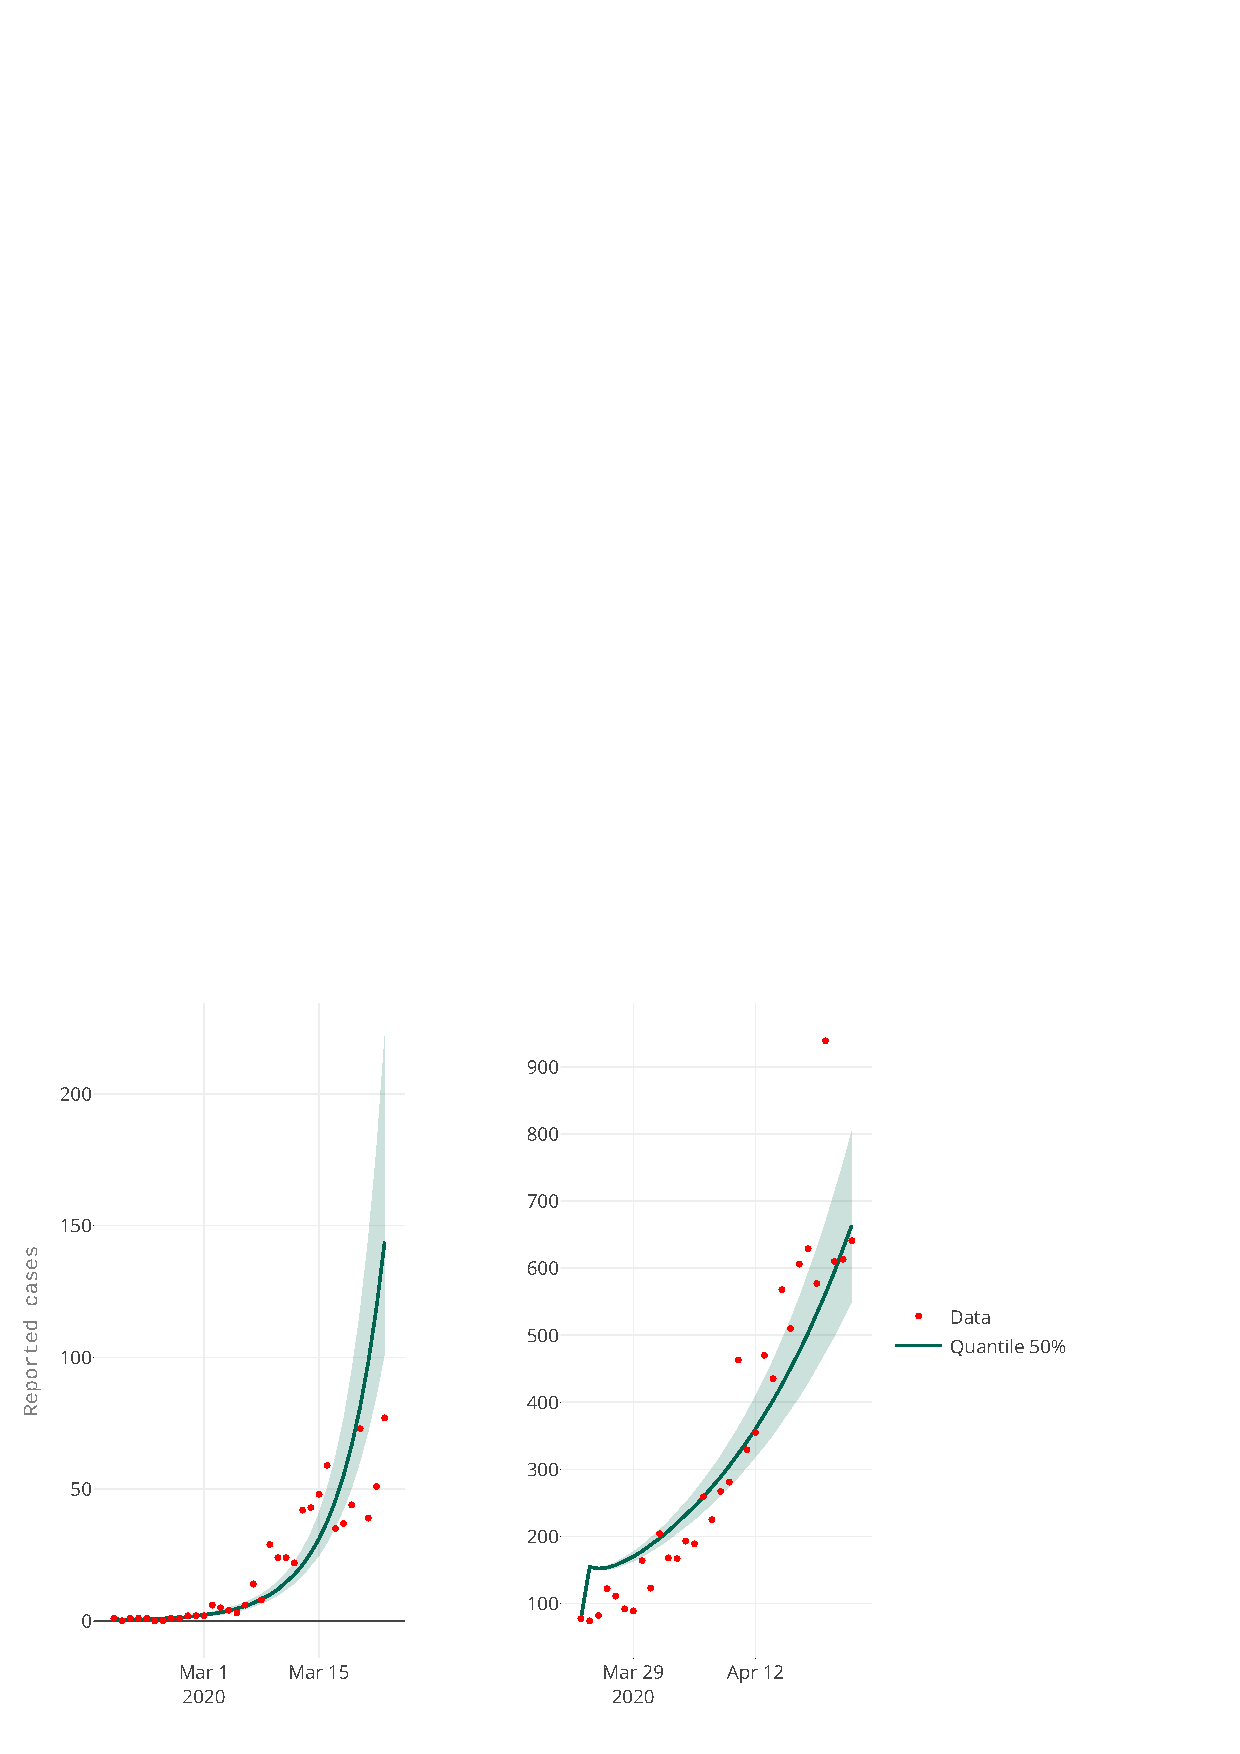
\includegraphics[scale=0.6, keepaspectratio]{FittingCurves.png}
    \caption{
        Fitting curves for the early phase of the COVID-19
        outbreak in Mexico City plus Mexico state.
        (A) Outbreak from February 19 to March 23, 2020.
        (B) Outbreak from March 23 to April 23, 2020.
        Reported data are shown in blue points, solid red line
        denote quantile 50 of all solutions
    }
    \label{Fig:fittingcurve}
\end{figure*}
%
\begin{table}[bth]
    \begin{center}
        \begin{tabular}{rl}
            \toprule
            Parameter & 95\% Confidence Interval
            \\
            \midrule
            $\beta_S$ & $[\num{0.2483712}, \num{0.48720714}]$ \\
            $\beta_A$ & $[\num{0.1851696}, \num{0.32181249}]$ \\
            $p$       & $[\num{0.061}, \num{0.2206}]$ \\
            $R_0$     & $[\num{1.702}, \num{1.887}]$\\
            \bottomrule
        \end{tabular}
        \caption{%
            Confidence interval for some parameters of system in
            \Cref{model1}, and for the basic reproductive number
            $(R_0)$.
        }\label{table_icparam4}
    \end{center}
\end{table}
%
On the other hand, since it is unclear when the vaccines will be available,
then we assume that our scenarios start on the growth stage of a second
outbreak (see \Cref{Fig:initial_conditions}) with the objective of starting
under a plausible scenario. Thus, for numerical results, initial conditions
normalized with total population
$N = \num{26446435}$, result
$S(0) = \num{0.463606046009872}$,
$E(0) = \num{0.00067033}$,
$I_S(0) = \num{0.00009283}$,
$I_A(0) = \num{0.00120986}$,
$R(0) = \num{0.532520194}$,
$D(0) = \num{0.00190074}$,
$V(0) = 0$, $X(0) = 0$, and
$Y_{I_{S}}(0) = \num{0.12258164}$.
\begin{figure*}[tbh]
    \centering
    \includegraphics[scale=0.6, keepaspectratio]{Is_dynamics.png}
    \caption{
        Dynamics of the symptomatic individuals. Black arrow indicates
        the outbreak stage in which we start our simulations.}
    \label{Fig:initial_conditions}
\end{figure*}
    \section{Imperfect-preventive Covid-19 vaccination}
      \input{vaccination_model}
    \section{Optimal controlled version}
       \input{cotrolled_version}

    \paragraph{Bayesian estimation}
%
    \section{Parameters}
      \begin{table*}
        \centering
        \begin{tabular}{@{}llr@{}}
        \toprule
            Parameter
            &   \centering{Median}
            &   Reference
            \\
            \midrule
              $q_r$, $\epsilon$
                &
                  \num{.4}, \num{.3}, \num{.1}
                &
                  this study
            \\
                $\beta_S$
                & $q_r \times \num{8.690483e-01} $
                & this study
            \\
                $\beta_A$
                & $q_r \times \num{7.738431e-01}$
                & this study
            
            \\
                $\kappa$
                & \num{0.19607843}
                & $*$
            \\
                $p$
                & \num{0.1213}
                & $*$
            \\
              $\theta$
              & \num{0.2},
              & this study
            \\
              $\delta_L$
              & \num{0.04}
              & postulated
            \\
                $\delta_H$
                &\num{0.2}
                & $*$
            \\
              $\delta_V$
              &\num{ 0.0027397260273972603}
              & $\delta_V ^{-1} = \SI{2}{years}$
            \\
            &&
                CanSinoBIO
            \\
              $\delta_R$
              & \num{0.00555556}
              & $\delta_R^{-1} \approx \SI{180}{days}$           
            \\
                $\mu$
                & \num{ 3.913894e-05}
                & $**$
            \\
                $\mu_{I_S}$
                & \num{0.0}
                & 
            \\
                $\mu_{H}$
                & \num{0.01632}
                & [FENG]
            \\
                $\gamma_S$
                & \num{0.09250694}
                & $*$
            \\
                 $\gamma_A$
                 & \num{0.16750419}
                 & $*$
            \\
               $\gamma_H$
                & \num{5.079869e-01}
                & $*$
            \\
              $\lambda_V$
              &  \num{0.00061135}
              &
            \\
              $\varepsilon$
              & \num{0.7}, \num{0.80}, \num{0.9}, \num{0.95}
              & [PRESS RELESASES]
            \\
            \midrule
                $N$
                 & \num{26446435}
                 & $**$
            \\
                $L_0$
                & \num{0.26626009702112796}
            \\
                $S_0$
                 & \num{0.463606046009872}
                 &
            \\
                $E_0$
                 & \num{0.00067033}
                 & $*$
            \\
                $I_{S_0}$
                & \num{9.283e-05}
                & $***$
            \\
                $I_{A_0}$
                & \num{0.00120986}
                & $*$
            \\
                $H_0$
                & \num{1.34157969e-04}
                & $**$
            \\
                $R_0$
                & \num{2.66125939e-01}
                &
            \\
                $D_0$
                & \num{0.00190074}
                & $**$
            \\
                $X_{vac}^0$
                & 0.0
            \\
                $V_0$
                & 0.0
            \\
                $Y_{I_S} ^ 0$ &
                \num{0.12258164}
            \\
                $B$
            &
                \num{0.0003592166581242425}
            &
                $
                    \displaystyle
                    \SI{9500}{beds} / {N}
                $
            \\
              $a_{I_S}$
                & \num{0.0020127755438256486}
                & DALY def
            \\
              $a_{H}$
                & \num{0.001411888738103725},
                or
            \\
            & $
                a_H(x):=
                \num{0.001411888738103725}
                \log(\frac{1}{B - \kappa I_S})
            $
            & DALY def [Jo 2020]
            \\
                $a_D$
                & \num{7.25}
                & DALY def
          \\
            \bottomrule
        \end{tabular}
    \end{table*}
    %
    \section{Optimal control problem}

    \section{Numerical Results}

    \paragraph{Bayesian}


    \section{Appendix}

Consider the following cost functional that we want to minimize
  \begin{equation}\label{costFunctional}
  \int_0^T C(t,X(t),u(t)) dt
  \end{equation}
subject to the dynamics
  \begin{equation}\label{dynamics}
  \dot{X}(t) = f(t,X(t),u(t)),  \qquad    0\leq t \leq T,
  \end{equation}
and the initial state $X(0)=x_0$. Let $t_0<t_1<\ldots <t_n$, with $t_0=0$ and $t_n=T$, be a partition of the interval $[0,T]$. We consider {\it piecewise constant controls} $\tilde{u}$ of the form
         \begin{equation}\label{PieceConstCont}
  \tilde{u}(t) = a_j\qquad t_j\leq t < t_{j+1}
         \end{equation}
 for $j=0,\ldots,n-1$.

{\sc Assumption 1}.


{\sc Assumption 2}.

By Assumption 1, the system
    \[    \dot{X}(t) = f(t,X(t),a_0), \quad X(0)=x_0, \qquad    0\leq t \leq t_1,
  \]
has a unique solution $\tilde{X}_0(t;x_0,a_0)$ which is continuous in $(x_0,a_0)$.  Next, put $x_1:=\tilde{X}_0(t_1;x_0,a_0)$ and consider the system
    \[    \dot{X}(t) = f(t,X(t),a_1), \quad X(t_1)=x_1, \qquad    t_1\leq t \leq t_2,
  \]
which, again by Assumption 1, has a unique solution $\tilde{X}_1(t;x_1,a_1)$ continuous in $(x_1,a_1)$. By following this procedure, we end up having a recursive solution
	\[  \tilde{X}_{n-1}(t;x_{n-1},a_{n-1}),\quad   x_{n-1}:=\tilde{X}_{n-2}(t_{n-1};x_{n-2},a_{n-1}),     \qquad    t_{n-1}\leq t \leq T. \]

Thus, for a control $\tilde{u}$ of the form \eqref{PieceConstCont} and the corresponding solution path $\tilde{X}$, we have
	\[
	\int_0^T C(t,\tilde{X}(t),\tilde{u}(t)) dt   =     \sum_{j=0}^{n-1}   \int_{t_j}^{t_{j+1}} C(t,\tilde{X}_j(t),a_j) dt.
	\]
Notice that each $\tilde{X}_j$ is a continuous function of $(a_0,\ldots,a_j)$	 and $x_0$. Therefore, by Assumption 2, the mapping
		\[
		(a_0,\ldots,a_{n-1}) \mapsto  \sum_{j=0}^{n-1}   \int_{t_j}^{t_{j+1}} C(t,\tilde{X}_j(t),a_j) dt
		\]
is continuous.

    \nocite{*}
    \bibliography{NovelCovid19.bib}
    \bibliographystyle{plain}
\end{document}
